% this file is called up by thesis.tex
% content in this file will be fed into the main document

%: ----------------------- name of chapter  -------------------------
\chapter{A Recurrent Neural Network Approach with Even Chance Training}\label{cp:endtoend}
\noindent
As recapped in Section~\ref{sec:2-rnnpm}, by far there are four types of ACE approaches:
\begin{itemize}
\item local feature extraction - global smoothing \cite{fujishima1999realtime,sheh2003chord}
\item local classification - global smoothing \cite{humphrey2012rethinking};
\item local feature learning - global classification - global smoothing \cite{boulanger2013audio,sigtia2015audio};
\item local feature learning - local classification - global smoothing \cite{zhou2015chord}.
\end{itemize}
All of these approaches incorporate a ``global smoothing'' stage after classification. This is a step that requires prior domain knowledge which does not belong to the deep learning framework. From a machine learning perspective, prior knowledge is considered suboptimal, because it is imposed by human engineers rather than learned by machines. It could also be suboptimal in terms of performance, if the machine learning model is powerful or the amount of training data is large enough. A machine learning system evolves by reducing the amount of prior knowledge involved while maintaining the overall system performances as much as possible.

Moreover, all existing approaches overlook the fact that the chords are distributed in a highly uneven way and that the chord classification problem is actually a skewed classes classification problem. If the similar approaches are used for LVACE, it is very probable that the systems will over-fit the chord types that are highly over-represented.

This Chapter presents an approach that on one hand employs a new neural network training scheme to achieve a more balanced performance on both common and uncommon chords, and on the other hand does not rely on ``global smoothing''.

Under the above taxonomy, the approach presented in this paper belongs to a new \textbf{``local feature extraction - global classification''} category. Instead of feature learning, it employs a normal feature extraction process, and the segmentation and classification processes are all done by one single RNN pass. To accommodate to large vocabulary, the RNN is trained via a skewed class oriented scheme. This scheme is shown to be very effective in improving the system's vocabulary versatility, compared with a scheme which does not attend to the skewed chord distribution.


%: ----------------------- contents from here ------------------------
\section{System Overview}\label{sec:4-sysover}
Figure \ref{fig:4-sysover} shows the system overview, which mainly contains a feature extraction module and a BLSTM-RNN sequence decoding module. The former is the same as the feature extraction process presented in Chapter~\ref{cp:ghmm}.

\begin{figure}[htb]
\centering
\includegraphics[width=0.4\columnwidth]{4/figures/sys.pdf}
\caption{BLSTM-RNN LVACE System Overview. The raw audio is feature extracted into a piece of chromagram or notegram, and then decoded by a BLSTM-RNN into a segmented chord sequence.}
\label{fig:4-sysover}
\end{figure}

\section{Implementation}\label{sec:4-blstm}
The key module in this system is the BLSTM-RNN. This section will first briefly discuss RNN's variable-length sequence training, and then elaborate on the implementation of the BLSTM-RNN.

\subsection{RNN Training}\label{sec:4-rnntrain}
An RNN can model the conditional probability of a label sequence $l$ given its corresponding input feature sequence $x$. Let's define the label alphabet as $L$, and let both $x$ and $l$ have the same length $T$ in the unit of time. The conditional probability $p(l|x)$ modeled by the RNN can be written as:

\begin{equation}\label{eq:4-rnnprob}
p(l|x) = \prod_{t=1}^T y_{l_t}^t  \quad\quad l\in L \quad and \quad |l| = |x|
\end{equation}

where $l_t$ is the $t^{th}$ element of $l$ and $y_{l_t}^t$ is the probability of predicting label $l_t$ at time $t$ given $x$. At time $t$, $y_{l_t}^t$ can also be written as $p(l_t|x)$, which is the value of the $l^{th}$ slot of RNN's prediction at time $t$. This RNN can be trained using a maximum likelihood approach by updating the network weights towards a direction that increases the conditional probability depicted in Equation~\ref{eq:4-rnnprob}. Thus this equation, or its logarithm, can be used as the objective function (cost function).

\subsection{BLSTM-RNN Architecture} \label{sec:4-blstmrnnarch}
Figure \ref{fig:4-blstm} shows the graphical model of the BLSTM-RNN used in this system framework, which has a forward and a backward hidden layer both with 800 LSTM units. The input layer has the same dimension as the input feature's. The output layer is a \textit{\#-chord-way} softmax layer. It takes a sequence of features as input, and generates a sequence of chord labels.

\begin{figure}[htb]
	\centering
	\includegraphics[width=0.6\columnwidth]{4/figures/blstm.pdf}
	\caption{The BLSTM-RNN. Both the forward and backward hidden layers contain 800 LSTM units}
	\label{fig:4-blstm}
\end{figure}

\subsection{Vocabulary and Datasets}
The large vocabulary supported by the proposed systems is again the \textit{SeventhsBass}. The datasets used in the experiments are the same as the Chapter~\ref{cp:ghmm}'s, but the data generation and augmentation schemes are different, which will be described as follows.

\subsection{Data Augmentation}
To generate training data, firstly all raw audios are transformed to chromagram and notegram representations. The original segment-wise ground truth annotations are upsampled to become frame-wise annotations with 1-to-1 mappings to their input representations. Due to the absence of phase information in chromagram and notegram, all data can be circularly transposed to 12 keys to yield 12 times the original amount of data \cite{humphrey2012rethinking}.

\subsection{Training and Cross-validation}
Two different training schemes are used. The only difference between them are the way of choosing training cases at each iteration:
\begin{itemize}
	\item completely random (CR): a random training case is chosen.
	\item even chance (EC): a training case starting with a certain chord type is chosen, and each chord type has an even chance to be chosen as the start.
\end{itemize}
The EC training scheme is inspired by the skewed class sensitive training methods \cite{chawla2004editorial}.
Considering a skewed distribution of chords in the training datasets \cite{burgoyne2011expert}, a random sampling scheme like CR will inevitably draw samples based on that same distribution, which causes lack of exposure of uncommon chords. The EC scheme, however, gives each class an equal chance of exposure during the training process. Concretely, the EC scheme is formalized as follows in Algorithm~\ref{alg:4-ectrain}:
\begin{algorithm}[h]
	\caption{EvenChanceTraining}
	\label{alg:4-ectrain}
	\begin{algorithmic}
		\REQUIRE
		training data set - $(X,y)$;
		number of chord classes - $nclass$;
		early stopping flag - $es$.
		\STATE % empty line
		\STATE $od$ = BalancedOrderedDict($y$, $nclass$)
		\STATE $iter$ = $0$
		\WHILE {not early-stopping}
		\IF {mod($iter$, $nclass$) is $0$}
		\STATE $coidx$ = random\_shuffle($0$:$nclass$-$1$)
		\ENDIF
		\STATE $tclist$ = $od(coidx_{mod(iter, nclass)})$
		\STATE draw a random item $e$ from $tclist$
		\STATE update network with $(X,y)_e$
		\STATE $iter$++
		\ENDWHILE
	\end{algorithmic}
\end{algorithm}

The core of this procedure is the ``\textit{BalancedOrderedDict}'' which generates a dictionary of \textit{(track index, chord change position)} tuples indexed by chord classes. It is formalized in Algorithm~\ref{alg:4-bod}, where each entry of $od$ contains a list of \textit{(track index, chord change position)} tuples.%This scheme guarantees an even chance of training for each class, given that each class has at least one case in the training set.
\begin{algorithm}[h]
	\caption{BalancedOrderedDict}
	\label{alg:4-bod}
	\begin{algorithmic}
		\REQUIRE
		labels of training data set - $y$;
		number of chord classes - $nclass$.
		\STATE % empty line
		\FOR {each class $i$ from $0$ to $nclass-1$}
		\STATE initialize an empty list $od[i]$
		\ENDFOR
		\FOR {each track index $j$ in $y$}
		\FOR {each frame poistion $k$ in $y[j]$} 
		\IF {$k$ is a chord change position}
		\STATE append ($j$,$k$) to $od[y[j][k]]$
		\ENDIF
		\ENDFOR
		\ENDFOR
		\RETURN
		$od$
	\end{algorithmic}
\end{algorithm}

The following describes the remaining training procedures that apply throughout the experiments. We try to report the precise settings of every parameter so that the readers may reproduce the results:
\begin{itemize}
	\item Each training case contains 500 frames of audio content with ground truth labels;
	%(subject to the end-of-track boundary condition)
	\item The network update signal is computed by an Adadelta optimizer \cite{zeiler2012adadelta};
	\item The training is regularized with dropout \cite{srivastava2014dropout} and early-stopping \cite{prechelt1998early};
	\item All dropout probabilities are set to 0.5;
	\item All early-stopping criteria are monitored using the validation error of the CNPop20 dataset, which is not in any cross-validation set; The validation cycle is 100 iterations;
	\item The model with the lowest validation loss will be saved; If the current validation loss is smaller than 0.996 of the best one, the early-stopping patience will increase by 0.3 times the current number of iterations;
	\item Training stops when the early-stopping patience is less than the current number of iterations.
\end{itemize}
For evaluation, five-fold cross-validation (CV) is performed throughout all experiments. Each fold is a combination of approximately 1/5 tracks of each dataset. Every model is trained on four folds and cross-validated on the remaining fold, resulting in a total number of five validation scores, the average of which will be the final scores to be reported.

\section{Results and Discussions} \label{sec:4-res}
This study evaluates several variants of the proposed approach (as summarized in Table~\ref{tab:4-varexplore}) in terms of the MIREX ACE standard metrics as well as the \textit{ACQA}. All the metric in this section are already introduced in Section~\ref{subsec:2-metrics}.
\begin{table}[htb]
	\caption{Variants considered in this study.}
	\centering
	\scriptsize
	\begin{tabular}{|c|c|c|} \hline
		Dimension & Configurations \\ \hline
		training scheme & completely random (CR); even chance (EC) \\ \hline
		data size & JK; JKU; JKUR; JKURB \\ \hline
	\end{tabular}
	\label{tab:4-varexplore}
\end{table}


\subsection{On Notegram Feature}
\Hsection{Sevenths, Inversions and ACQA}
Table~\ref{tab:4-acqa-ns} shows the comparison between CR and EC training schemes on some uncommon (\textit{non-majmin}) \cite{burgoyne2011expert} chords' \textit{WCSR}s as well as the \textit{ACQA}. The six chord types in the table are chosen because they have relatively more weights in pop/rock songs than the more long-tail ones such as \textit{min/5} and \textit{min/b3}. Note that \textit{maj/5} and \textit{maj/3} are also included in two other large vocabularies proposed by Mauch \cite{mauch2010automatic} and Cho \cite{cho2014improved}.
\begin{table}[htb]
	\caption{Comparison between CR and EC: seventh chords, inversions and ACQA scores; Dataset: JKURB}
	\centering
	\scriptsize
	\begin{tabular}{|c|c|c|c|c|c|c|c|} \hline
		& \textit{maj7} & \textit{7} & \textit{min7} & \textit{maj/5} & \textit{maj/3} & \textit{7/b7} & \textit{ACQA} \\ \hline
		CR & 7.3 & 6.6 & 24.1 & 4.5 & 24.5 & 0.0 & 10.8 \\ \hline
		EC &  14.6 & 9.9 & 30.9 & 12.0 & 32.4 & 7.8 & 13.2 \\ \hline
	\end{tabular}
	\label{tab:4-acqa-ns}
\end{table}

The results show that EC outscores CR in all categories, some of which by very large amount such as \textit{maj/5} and \textit{maj/3}. Although not all chord types' results are shown, the \textit{ACQA} results suggest that the EC training scheme could lead to a much more balanced LVACE system under a skewed class distribution.

\begin{figure}[htb]
	\centering
	\includegraphics[scale=0.4,trim={0cm 6cm 0cm 6cm},clip]{4/figures/ftacqa-ns.pdf}
	\caption{Multiple comparison test on ACQAs}
	\label{fig:4-ftacqa-ns}
\end{figure}
We perform a Friedman test on the track-wise \textit{ACQA} results of both systems. After that we use the Tukey HSD (honest significant difference) to perform a multiple comparison test on the Friedman test's statistics with a significance level of 0.05. The results as shown in Figure~\ref{fig:4-ftacqa-ns} confirm that EC is significantly better than CR in \textit{ACQA}.

\Hsection{Major, Minor and WCSR}
The EC trained system has a more balanced performance than the CR's, however, it scarifies common chords' \textit{WCSR}s. Table~\ref{tab:4-wcsr-ns} shows the comparison between CR and EC on some common (\textit{majmin}) \cite{burgoyne2011expert} chords' \textit{WCSR}s as well as on the overall \textit{SeventhsBass} \textit{WCSR}.
\begin{table}[htb]
	\caption{Comparison between CR and EC: major, minor and WCSR scores; Dataset: JKURB}
	\centering
	\scriptsize
	\begin{tabular}{|c|c|c|c|} \hline
		& \textit{maj} & \textit{min} & \textit{WCSR} \\ \hline
		CR & 74.2 & 52.2 & 52.0 \\ \hline
		EC &  67.8 & 51.4 & 50.6 \\ \hline
	\end{tabular}
	\label{tab:4-wcsr-ns}
\end{table}

Although the two schemes have very close scores on \textit{min}, there is a large difference in \textit{maj}. Due to the dominantly large weight of \textit{maj} chords in the JKURB dataset combination, it eventually leads to CR's much higher \textit{WCSR}, despite EC performs better in most of the other chord types. CR's much higher \textit{maj} \textit{WCSR} is not unexpected: since it draws each training case at random, the probability that each chord type gets ``seen'' by the neural net is subject to the distribution of chord types in the training dataset, and therefore the \textit{maj} chords are ``learned'' much more than the other chords.

\begin{figure}[h!]
	\centering
	\includegraphics[scale=0.4,trim={0cm 6cm 0cm 6cm},clip]{4/figures/ftwcsr-ns.pdf}
	\caption{Multiple comparison test on WCSRs}
	\label{fig:4-ftwcsr-ns}
\end{figure}
We perform a Friedman test on the track-wise \textit{WCSR} results of both systems. After that we use the Tukey HSD to perform a multiple comparison test on the Friedman test's statistics with a significance level of 0.05. The results as shown in Figure~\ref{fig:4-ftwcsr-ns} confirm that CR is significantly better than EC in \textit{WCSR}.

\Hsection{On Different Datasets}
For more convincing comparison results, the same experiment is run 4 times using different dataset combinations. Table~\ref{tab:4-datasize-ns} shows the results of JK, JKU, JKUR and JKURB. We only report the \textit{WCSR} and \textit{ACQA} for brevity.
\begin{table}[htb]
	\caption{Comparison between CR and EC: WCSR and ACQA on different datasets.}
	\centering
	\scriptsize
	\begin{tabular}{|c|c|c|c|c|} \hline
		& CR-WCSR & EC-WCSR & CR-ACQA & EC-ACQA \\ \hline
		JK & 46.4 & 46.4 & 13.5 & 15.5 \\ \hline
		JKU & 50.4 & 49.1 & 11.2 & 13.5 \\ \hline
		JKUR & 50.1 & 49.6 & 12.8 & 14.5 \\ \hline
		JKURB & 52.0 & 50.6 & 10.8 & 13.2 \\ \hline
	\end{tabular}
	\label{tab:4-datasize-ns}
\end{table}

In all these experiments, the EC systems get higher \textit{ACQA}s, but lower or equal \textit{WCSR}s, than the CR systems. It is sufficient to say that EC is better at training a balanced performing LVACE system under skewed class distribution, while CR is better at training an LVACE system with higher overall performance.

For both training schemes, the increment of training data will lead to the increase of \textit{WCSR}, but the same thing does not happen in \textit{ACQA}. Assuming that every dataset contains a certain amount of noise (i.e., mis-labeled or mis-segmented chord regions), this observation could be tentatively explained as follows. \textit{WCSR} is mostly relying on the quality of \textit{majmin} chord labels, which are on average easier to be labeled. Therefore the increment of data will also increase the \textit{WCSR} score. \textit{ACQA}, however, is mostly relying on the quality of \textit{non-majmin} chord labels, which are on average more difficult to be labeled. Therefore the increment of data could not guarantee the increase of \textit{ACQA} score, since it is hard to guarantee the proportion of \textit{non-majmin} noise in the incremental data is smaller than those of the original data.

\subsection{On Chromagram Feature}\label{sec:4-ch}
\Hsection{Overall Performances}\label{sec:4-over-ch}
\begin{table}[htb]
	\caption{WCSRs of different system variants.}
	\label{tab:4-overallres}
	\centering
	\scriptsize
	\begin{tabular}{|c|c|c|c|c|c|c|c|c|}\hline
		System & \textit{MajMin} & \textit{MajMinBass} & \textit{Sevenths} & \textbf{\textit{SeventhsBass}} & \textit{Segmentation Quality}  \\ \hline
		CR-JK & 67.1 & 65.0 & 49.7 & 48.2 & 78.1 \\ \hline
		EC-JK & 68.0 & 65.2 & 51.3 & 49.3 & 77.3 \\ \hline
		CR-JKU & 67.4 & 65.6 & 54.9 & 53.4 & 76.9 \\ \hline
		EC-JKU & 67.7 & 65.9 & 55.3 & 53.7 & 76.3 \\ \hline
		CR-JKUR & 70.1 & 68.3 & 56.8 & \textbf{55.2} & 78.0 \\ \hline
		EC-JKUR & 70.0 & 68.1 & 56.6 & 55.0 & 76.9 \\ \hline
		CR-JKURB & 70.6 & 68.7 & 56.3 & 54.7 & 78.0 \\ \hline
		EC-JKURB & 70.1 & 68.2 & 57.6 & \textbf{56.0} & 76.8 \\ \hline
	\end{tabular}
\end{table}
Table~\ref{tab:4-overallres} shows the overall \textit{WCSR}s of systems implemented with both training schemes. Note that the \textit{SeventhsBass} column represents the true evaluation score under the \textit{SeventhsBass} vocabulary, while the other three columns to the left are scores with certain types of chord confusion tolerance.

Along the \textit{SeventhsBass} column, there is a trend that for both training schemes, system performances increase with more training data. When the data set is fixed, the EC systems' \textit{SeventhsBass} score are fairly comparable or slightly higher than the CR systems'. The same trend is also observed in columns of \textit{MajMin}, \textit{MajMinBass} and \textit{Sevenths}.

For \textit{segmentation quality}, CR systems are found to be consistently scoring slightly higher than the EC systems. Note that CR draws a training case from a random starting point which could be in the middle of a segment, while EC always draws a case from the start of a segment. We speculate this deviation eventually leads to the CR systems' more exposure to segment boundaries during training, and thus they have a slightly better ``understanding'' of segments.

\Hsection{Balanced performances} \label{sec:4-scper}
\begin{table}[htb]
	\caption{Some uncommon chords' WCSRs and the ACQAs}
	\label{tab:4-ltres}
	\centering
	\scriptsize
	\begin{tabular}{|c|c|c|c|c|c|c|c|c|}\hline
		System & \textit{maj/5} & \textit{maj/3} & \textit{7/b7} & \textit{ACQA}\\ \hline
		CR-JK & 17.9 & 43.2 & 28.9 & 16.6\\ \hline
		EC-JK & 23.3 & 42.7 & \textbf{37.2} & 19.7\\ \hline
		CR-JKU & 11.9 & 36.5 & 10.1 & 15.0\\ \hline
		EC-JKU & 20.3 & 40.2 & 35.4 & 19.2\\ \hline
		CR-JKUR & 18.8 & 46.0 & 7.0 & 16.6\\ \hline
		EC-JKUR & \textbf{23.7} & \textbf{50.0} & 32.4 & \textbf{20.9}\\ \hline
		CR-JKURB & 11.9 & 38.5 & 4.9 & 14.7\\ \hline
		EC-JKURB & 18.7 & 42.2 & 24.0 & 18.4\\ \hline
	\end{tabular}
\end{table}
Table~\ref{tab:4-ltres} shows the systems' performances on some important uncommon chords' \textit{WCSR}s and the \textit{ACQA}. These three chord types (i.e. $maj/5$, $maj/3$ and $7/b7$) are most commonly used in pop/rock songs among all uncommon chords in the \textit{SeventhsBass} vocabulary. We could notice obvious performance advantages of EC in all these categories under the same amount of training data sizes.

For \textit{ACQA}, again, we see that all EC systems have clear advantages over CR systems. This demonstrates that the EC training scheme can improve the vocabulary versatility of an ACE system.

It should be pointed out that in Table~\ref{tab:4-ltres} neither the \textit{WCSR} of a specific chord nor the \textit{ACQA} is proportional to the amount of training data. Figure~\ref{fig:4-datavsmaj3} and ~\ref{fig:4-datavsmaj5} show the \textit{WCSR} trends of \textit{maj/3} and \textit{maj/5} chords. They all have local maximum at JK and JKUR and local minimum at JKU and JKURB.

\pgfplotsset{width=10cm,height=6cm,every node near coord/.append style={font=\scriptsize}}
\begin{figure}[htb]
	\centering
	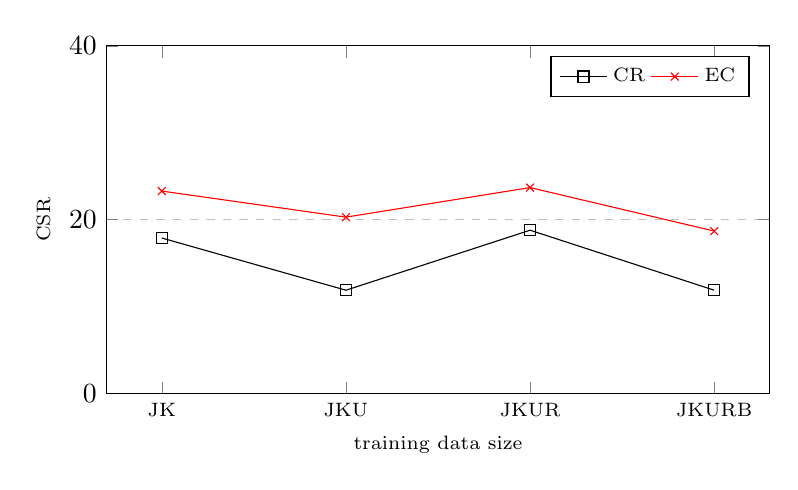
\begin{tikzpicture}
	\begin{axis}[
	title={},
	title style = {font=\scriptsize},
	xlabel={training data size},
	x label style={font=\scriptsize},
	x tick label style={font=\scriptsize},
	xtick=data,
	ylabel={CSR},
	y label style={font=\scriptsize},
	ymin=0, ymax=40,
	symbolic x coords={JK, JKU, JKUR, JKURB},
	ytick={0,20,40},
	legend pos=north east,
	legend style={legend columns=-1, font=\scriptsize},
	ymajorgrids=true,
	grid style=dashed,
	]
	
	\addplot[
	color=black,
	mark=square,
	]
	coordinates {
		(JK,17.9)(JKU,11.9)(JKUR,18.8)(JKURB,11.9)
	};
	
	\addplot[
	color=red,
	mark=x,
	]
	coordinates {
		(JK,23.3)(JKU,20.3)(JKUR,23.7)(JKURB,18.7)
	};
	\legend{CR, EC} 
	\end{axis}
	\end{tikzpicture}
	\caption{$maj/3$ performance v.s. training data size}
	\label{fig:4-datavsmaj3}
\end{figure}
\pgfplotsset{width=10cm,height=6cm,every node near coord/.append style={font=\scriptsize}}
\begin{figure}[htb]
	\centering
	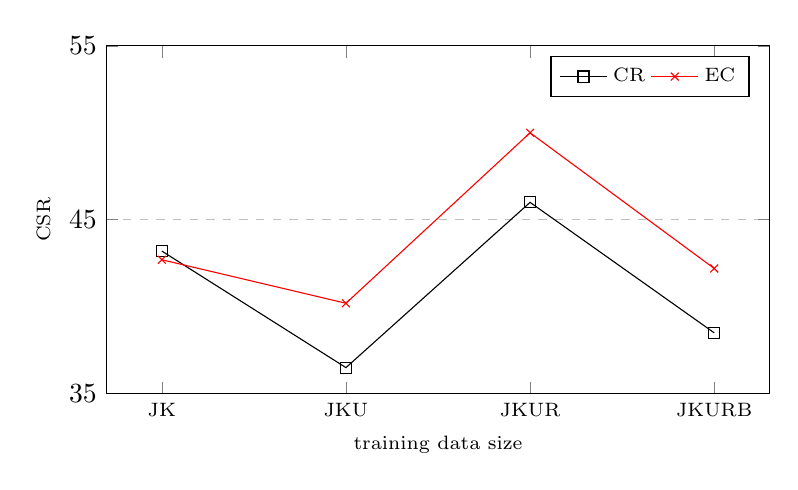
\begin{tikzpicture}
	\begin{axis}[
	title={},
	title style = {font=\scriptsize},
	xlabel={training data size},
	x label style={font=\scriptsize},
	x tick label style={font=\scriptsize},
	xtick=data,
	ylabel={CSR},
	y label style={font=\scriptsize},
	ymin=35, ymax=55,
	symbolic x coords={JK, JKU, JKUR, JKURB},
	ytick={35,45,55},
	legend pos=north east,
	legend style={legend columns=-1, font=\scriptsize},
	ymajorgrids=true,
	grid style=dashed,
	]
	
	\addplot[
	color=black,
	mark=square,
	]
	coordinates {
		(JK,43.2)(JKU,36.5)(JKUR,46.0)(JKURB,38.5)
	};
	
	\addplot[
	color=red,
	mark=x,
	]
	coordinates {
		(JK,42.7)(JKU,40.2)(JKUR,50.0)(JKURB,42.2)
	};
	\legend{CR, EC} 
	\end{axis}
	\end{tikzpicture}
	\caption{$maj/5$ performance v.s. training data size}
	\label{fig:4-datavsmaj5}
\end{figure}

Table~\ref{tab:4-chorddist} shows the distribution of common chords (majmin) and uncommon chords (sevenths and inversions) in the datasets we use. We see that the datasets U and B have more uneven distributions of common and uncommon chords than dataset R, and therefore when they are mixed up with other data, the overall amount of uncommon chords' exposure will be decreased. This explains the CR's curve in Figure~\ref{fig:4-datavsmaj5}.
\begin{table}[h]
	\centering
	\scriptsize
	\caption{Distribution of chords in the datasets}
	\label{tab:4-chorddist}
	\begin{tabular}{|c|c|c|c|}\hline
		Dataset & majmin\% & sevenths\% & inversions\%\\ \hline
		C & 58.7 &	28.6 & 12.7\\ \hline
		J & 47.4 & 31.7 & 20.9\\ \hline
		K & 66.9 & 21.8 & 11.4\\ \hline
		U & 69.8 & 21.7 & 8.4\\ \hline
		R & 58.1 & 32.5 & 9.4\\ \hline
		B & 81.9 & 12.1 & 6.0\\ \hline
	\end{tabular}
\end{table}
For EC, each chord type has an even chance to be chosen as the start of a training case. Each training case has 500 frames, which contains multiple chords. Because of this, there is still uneven distribution of common and uncommon chords during the training process. The EC scheme in effect only boosts the exposure of uncommon chords to a certain level, but could not make the chances of common and uncommon chords totally even. Therefore, the same reason for CR also apply to explain EC's curve in Figure~\ref{fig:4-datavsmaj5}.


\subsection{Baseline Comparison}

\Hsection{SeventhsBass Evaluation}
\begin{table}[htb]
	\caption{Comparison between our systems and Chordino - overall performance; The systems are trained using JKURB}
	\label{tab:4-cpcd}
	\centering
	\scriptsize
	\begin{tabular}{|c|c|c|c|c|c|c|c|c|c|c|c|c|c|}\hline
		System & \textit{MajMin} & \textit{MajMinBass} & \textit{Sevenths} & \textbf{\textit{SeventhsBass}} & \textit{Segmentation Quality}\\ \hline
		CR-ch & 70.6 & 68.7 & 56.3 & 54.7 & 78.0\\ \hline
		EC-ch & 70.1 & 68.2 & \textbf{57.6} & \textbf{56.0} & 76.8\\ \hline
		Chordino & \textbf{72.4} & \textbf{69.1} & 55.8 & 52.8 & \textbf{83.8}\\ \hline
	\end{tabular}
\end{table}

Finally, we compare the proposed LVACE approach with the baseline approach - Chordino\cite{cannam2013mirex}. It has a similar feature extraction module as the proposed approach and it supports a similar set of large vocabulary. Chordino is an LVACE system that represents the state-of-the-art in terms of the \textit{ACQA}.

Table~\ref{tab:4-cpcd} shows the comparison, in which we select two systems trained with the largest possible amount of data with different training schemes. In terms of \textit{WCSR}s, our systems slightly outperform Chordino in \textit{Sevenths} and \textit{SeventhsBass} scores, but underperform Chordino in the more relaxed \textit{MajMin} and \textit{MajMinBass} scores.

\begin{figure}[h!]
	\centering
	\includegraphics[scale=0.4,trim={0cm 6cm 0cm 6cm},clip]{4/figures/ftwcsr-ch.pdf}
	\caption{Multiple comparison test on SeventhsBass WCSRs}
	\label{fig:4-ftwcsr-ch}
\end{figure}
Of all the categories in Table~\ref{tab:4-cpcd}, \textit{SeventhsBass} represents the large vocabulary metric. We therefore perform a Friedman test on the track-wise SeventhsBass \textit{WCSR} results of the three systems. After that we use the Tukey HSD (honest significant difference) to perform a multiple comparison test on the Friedman test's statistics with a significance level of 0.0. The results are shown in Figure~\ref{fig:4-ftwcsr-ch}, which confirm that both CR and EC are significantly better than Chordino in SeventhsBass \textit{WCSR}, and there is no significant difference between CR and EC.

A large difference is found in \textit{segmentation quality}, in which Chordino scores 5.3 and 7 points higher than our systems. As noted previously, the \textit{segmentation quality} is indeed a problem in this approach. One could expect boosts of overall performance as well as balanced performance if the \textit{segmentation quality} score could be raised to at least the Chordino's level.

\Hsection{Uncommon Chords and ACQA}
\begin{table}[htb]
	\caption{Comparison between our systems and Chordino - uncommon and balanced performance; The systems are trained using JKURB}
	\label{tab:4-cpcd-2}
	\centering
	\scriptsize
	\begin{tabular}{|c|c|c|c|c|c|c|c|c|c|c|c|c|c|}\hline
		System & \textit{maj/5} & \textit{maj/3} & \textit{7/b7} & \textit{ACQA} \\ \hline
		CR-ch & 11.9 & 38.5 & 4.9 & 14.7\\ \hline
		EC-ch & 18.7 & \textbf{42.2} & 24.0 & \textbf{18.4}\\ \hline
		Chordino & \textbf{ 27.6} & 29.8 & \textbf{24.4} & \textbf{20.9}\\ \hline
	\end{tabular}
\end{table}
Table~\ref{tab:4-cpcd-2} shows another set of comparisons in terms of uncommon chords' \textit{WCSR}s and the \textit{ACQA}. The CR system underperforms Chordino in all the categories except for $maj/3$.	The EC system outperforms Chordino in $maj/3$ and is close to Chordino in both $7/b7$ and \textit{ACQA}.

\begin{figure}[h!]
	\centering
	\includegraphics[scale=0.4,trim={0cm 6cm 0cm 6cm},clip]{4/figures/ftacqa-ch.pdf}
	\caption{Multiple comparison test on ACQAs}
	\label{fig:4-ftacqa-ch}
\end{figure}
We perform a Friedman test on the track-wise \textit{ACQA} results of the three systems. After that we use the Tukey HSD to perform a multiple comparison test on the Friedman test's statistics with a significance level of 0.05. The results are shown in Figure~\ref{fig:4-ftacqa-ch}, which indicate that both EC and Chordino are significantly better than CR in \textit{ACQA}, and there is no significant difference between EC and Chordino.

\section{Summary}\label{sec:4-concln}
%This chapter proposes a ``local feature extraction - global classification'' BLSTM-RNN based LVACE system that supports SeventhsBass vocabulary. This system has a handcrafted feature extraction process, and can be compared with Chordino in a statistically fair way. To cater for large vocabulary recognition, an even chance training scheme is designed. Several variants of the system are trained and implemented.
This Chapter presents a BLSTM-RNN based LVACE system, trained using a skewed class oriented ``even chance'' scheme. Several system variants with different configurations are implemented and evaluated using both notegram and chromagram features as input.

According to the notegram's results, the EC training scheme is superior in both the uncommon (\textit{non-majmin}) chords' \textit{WCSR}s and the \textit{ACQA}, at the expense of the common (\textit{majmin}) chords' \textit{WCSR}s and the overall \textit{WCSR}. While according to the chromgram's results the EC training scheme can improve uncommon chords' \textit{WCSR}s as well as the \textit{ACQA}, while still maintaining the overall \textit{WCSR} performance at the level of the CR training scheme.

When compared with Chordino, the EC system's performance is still very competitive since it significantly outperforms Chordino in \textit{SeventhsBass} \textit{WCSR}, and it does not significantly differ from Chordino in \textit{ACQA}. However, the EC systems suffer from bad \textit{segmentation quality}, which should be well noted as the biggest drawback for the proposed LVACE approach in this paper. Improving the \textit{segmentation quality} may require a more focused learning strategy towards chord segmentation.

Extrapolating from this work, the future LVACE researches, in a deep learning perspective, should focus on at least the following three aspects/challenges:
\begin{itemize}
	\item implementing deeper models
	\item embracing ground truth subjectivity
	\item improving accuracy on uncommon and long-tail chords
\end{itemize}

\Hsection{Deeper Models}
The first aspect considers using a deeper model for sequence modeling. This is rather a challenge motivated by pure scientific interest than practical interest. This paper describes a BLSTM-RNN that models sequence transformation from chromagram to segmented chord sequence. But as we know, the promise of deep learning is to extract useful features from raw input, and to learn better transformations than handcrafted transformations. Thus this challenge asks for a deep learning model in a truly ``end-to-end'' sense, that captures every transformation from waveform level all the way to segmented chord sequence level. Such a model might not outperform the state-of-the-art at the beginning, but might show promising potentials to achieve the optimal performance in the long run.

\Hsection{Subjectivity Issue}
The second challenges are fundamental to all kinds of machine learning researches, and it is especially non-neglectable in LVACE research, since human chord annotators may disagree a lot, especially in uncommon and long-tail chords. As a result, some researchers doubt the necessity to estimate uncommon and long-tail chords. Such opinions may have their merit under certain circumstances, particularly when they are referring to an ACE system built for chord learning beginners. However, they are not justified under a more practical scenario, where people need more ``accurate'' chord annotations for busking, practicing or rehearsal.

Therefore the annotation subjectivity issue needs to be embraced, or resolved, rather than neglected or abandoned. This is a difficult topic that may demand a lot of work and intelligence from data science, statistics, and machine learning. One key observation is that human learns to annotate chords by reading and listening to a lot of different examples, regardless of the annotators. When a person reaches a certain level, s/he may be able to correct the wrong annotations. The more advanced s/he is, the more uncommon and long-tail chords s/he is able to annotate, spot and correct.

But this issue should not overrule another equally important issue: to build a machine that ``learns well''. A 100\% ``golden standard'' ground truth should not be a necessary premise for building any machine learning system. Should there be any chaos or noise, the research community could always regress to use annotations from one single annotator.

\Hsection{Uncommon Chords Accuracy}
The uncommon chords accuracy is always interleaved with subjectivity issue. But it should be noted that not all instances of all uncommon chord types are subjected to the annotation subjectivity. Although currently there is not any statistics showing the exact relationship between them, musical experience told us that some uncommon chord instances are much easier to be recognized than others, thus they receive less disagreement among annotators.

%Evaluation results show some variants largely outperform Chordino in terms of large vocabulary scores, and they are almost as good as Chordino in terms of small vocabulary scores, despite having much worse segmentation qualities. It can be concluded that the proposed BLSTM-RNN architecture is better than the dedicated handcrafted GMM-HMM in terms of large vocabulary sequence modeling, but it suffers from bad sequence segmentation.

%Through detail analysis of the results, a plausible issue of annotation inconsistency is identified. As suggested in Chapter~\ref{cp:background}, a workaround would be to always use annotations provided by one single source/annotator, or, to the other extreme, always use multiple annotators and apply majority vote or data fusion. But eventually, the ultimate evaluation tool may remain a fully subjective one, that let user experience to judge system performance.

%Even chance training has been demonstrated very efficient in improving long-tail symbol recalls. It also boosts some very long-tail cases from zero score to non-zero. However, it sacrifices the performances of large population chords, and thus downgrades the overall performances in all but the versatility category.

%To improve this system, the key thing to be done is to improve RNN's segmentation quality, since it determines an upper-bound of all other system performance, and the scores of all other metrics scale in proportion to segmentation quality. This can possibly be done through a dedicated segmentation training pass, a deeper RNN model, or combination of a segmentation-RNN with a annotation-RNN in a hierarchical way.




% ---------------------------------------------------------------------------
%: ----------------------- end of thesis sub-document ------------------------
% ---------------------------------------------------------------------------

